%=================================================
%% 2 percentage signs represent comments for code;
% 1 percentage sign represents commented out code

%% Beamer template for presentations
%% Colour palette chosen with colour blindness in
%% mind: https://davidmathlogic.com/colorblind/
%% Paul L. Tran
%% Last updated: 05 Oct, 2025
%=================================================

%=================================================
\documentclass[aspectratio = 1610, english, 11pt, xcolor = dvipsnames]{beamer}

%% Loading packages
\usepackage{lmodern}
\usepackage{newtxmath}
\usepackage{amsthm}
\usepackage{microtype}
\usepackage[T1]{fontenc}
\usepackage{booktabs}
\usepackage{mathtools}
\usepackage{graphicx}
\usepackage{multirow}
\usepackage{enumerate}
\usepackage{multicol}
\usepackage{makecell}
\usepackage{adjustbox}
\usepackage{varwidth}
\usepackage{tabularx}
\providecommand{\tabularnewline}{\\}
\usepackage{centernot}
\usepackage{tikz}
\usetikzlibrary{shapes, arrows, matrix, chains, positioning, decorations.pathreplacing, decorations.pathmorphing, backgrounds, tikzmark, nef}
\tikzset{input node/.style={circle, draw, fill=gray!20, minimum size=1cm},
  hidden node/.style={circle, draw=blue!50, fill=blue!20, minimum size=1cm},
  output node/.style={circle, draw=cyan!50, fill=cyan!20, minimum size=1cm},
  arrow/.style={->, >=stealth}
}
\usepackage[
  sorting = nyt,
  citestyle = authoryear,
  bibstyle = authoryear-comp,
  defernumbers = true,
  maxnames = 2,
  minnames = 1,
  maxbibnames = 99,
  giveninits = false,
  bibencoding = utf8,
  terseinits = true,
  uniquename = init,
  dashed = false,
  doi = true,
  isbn = false,
  natbib = true,
  backend = biber,
  date = year
]{biblatex}

%% Setting base theme
\usetheme{Frankfurt}

%% Customising theme and alert colours according to IBM's design palette for colour blindness (https://davidmathlogic.com/colorblind/)
\definecolor{basecolor}{RGB}{100, 143, 255} % HEX #648fff
\colorlet{darkbasecolor}{basecolor!60!black} % Section header slightly darker
\definecolor{alertcolor}{RGB}{181, 53, 116} % HEX #b53574
\setbeamercolor{alerted text}{fg = alertcolor}

%% Assigning colours to the theme
\usecolortheme[named = basecolor]{structure}
\setbeamercolor{section in head/foot}{fg = white, bg = darkbasecolor}

%% Setting title page style
\setbeamertemplate{title page}[default][colsep = -4bp, shadow = false]

%% Setting frame title style
\setbeamertemplate{frametitle}{
  \nointerlineskip
  \begin{beamercolorbox}[sep = 0.2cm, ht = 1.8em, wd = \paperwidth, shadow = False]{frametitle}
    %% Removing \insertframetitle from tikzpicture environment due to the latter causing issues with
    %% \hfill in the frame titles
    \insertframetitle
    % \begin{tikzpicture}[overlay, remember picture]
    %   \node[anchor = west, align = left] at (-0.2, 0.17){\insertframetitle};
    % \end{tikzpicture}
  \end{beamercolorbox}
}

%% Creating command to widen slide contents
%% Format: \Wider[measurement]{Slide contents}
\newcommand\Wider[2][3em]{%
  \makebox[\linewidth][c]{%
    \begin{minipage}{\dimexpr\textwidth+#1\relax}
      \raggedright#2
    \end{minipage}
  }
}

%% Making spacing shortcuts if feeling lazy
\newcommand{\bs}{\bigskip{}}
\newcommand{\ms}{\medskip{}}

%% Setting header style (with sections)
\setbeamertemplate{headline}{
  \begin{beamercolorbox}{section in head/foot}
    \vskip2pt\insertsectionnavigationhorizontal{\paperwidth}{}{}\vskip2pt
  \end{beamercolorbox}
}

%% Setting footer style
% To remove the navigation symbols from the bottom of slides
\setbeamertemplate{navigation symbols}{} 

%% Storing original definition of \insertframenumber so that when certain
%% slides have their frame numbers ignored in the count and are hidden, the PDF
%% metadata isn't affected. Specifically, hiding and not counting certain slides uses:
%% \begingroup \def\insertframenumber{\texorpdfstring{\relax}{\sidepanenumber}} \endgroup
\let\sidepanenumber\insertframenumber

%% Customising footer
\setbeamertemplate{footline}{
  \hbox{
    \setbeamercolor{footercolor}{bg = white, fg = white!50!black}
    \begin{beamercolorbox}[wd = 0.333333\paperwidth,ht = 2.25ex, dp = 2ex, left]{footercolor}%
      \hspace*{2ex} \insertshortauthor\hspace*{0.5ex}  (\insertshortinstitute)
    \end{beamercolorbox}%
    \begin{beamercolorbox}[wd = 0.333333\paperwidth,ht = 2.25ex, dp = 2ex, center]{footercolor}%
      \insertshorttitle
    \end{beamercolorbox}%
    \begin{beamercolorbox}[wd = 0.333333\paperwidth,ht = 2.25ex,dp = 2ex,right]{footercolor}%
      \insertframenumber{}
      %% Uncomment the line below if you wish to show the total frame number
      / \inserttotalframenumber
      \hspace*{4ex} 
    \end{beamercolorbox}
  }
  \vskip0pt
}

%% Setting bullet shapes
%% Default bullet shapes are [default, circle, square]
%% Using non-default shape. like a dash, require the format {--}
\setbeamertemplate{enumerate items}[default]
\setbeamertemplate{itemize item}[triangle]
\setbeamertemplate{itemize subitem}[circle]
\setbeamertemplate{itemize subsubitem}{--}
\setbeamertemplate{section in toc}[circle]

%% Setting footnote size
\setbeamerfont{footnote}{size = \tiny}
\renewcommand*{\thefootnote}{\fnsymbol{footnote}}

%% Setting covered items in slides to be transparent
\setbeamercovered{transparent}

%% Enabling numbered captions for tables and figures
\setbeamertemplate{caption}[numbered]
%=================================================

%=================================================
%% Creating title
\newcommand\makebeamertitle{\frame{\maketitle}}
\title[Short Title]{\textbf{Title}\\Subtitle}
\author[Surname]{Name Surname\thanks{Email: \href{mailto:your@email.address}{your@email.address}. Website: \href{https://google.com/}{https://yourwebsite.com/}.}}
\institute[Institution]{Institution} 
\date{
  This version: \today\\
  \begin{center}
    {\small \href{https://github.com/paultran47/beamertemplate}{\alert{[Click here for the latest version]}}}
  \end{center}
}
%=================================================

%=================================================
%% Creating references
\addbibresource{mybib.bib}

%% Removing document icons from references
\setbeamertemplate{bibliography item}{}

%% Making URL the same font as text, not courier default
\urlstyle{same}
\newcommand{\doi}[1]{\url{#1}}

%% Changing font of biblatex acronyms into all caps since lmodern doesn't have small caps (e.g., DOI). Default font size is \tiny
\renewcommand*{\mkbibacro}[1]{#1}

\makeatletter
%% Setting up footnote to work in the align environment
\let\original@footnote\footnote
\newcommand{\align@footnote}[1]{
  \ifmeasuring@
    \chardef\@tempfn = \value{footnote}
    \footnotemark
    \setcounter{footnote}{\@tempfn}
  \else
    \iffirstchoice@
      \original@footnote{#1}
    \fi
  \fi
}
\pretocmd{\start@align}{\let\footnote\align@footnote}{}{}
\makeatother
%=================================================

%=================================================
%% Creating slides
\begin{document}
  \section{Introduction}
  \begin{frame}
    \maketitle
  \end{frame}

  \begin{frame}{Introduction}
    \begin{itemize}
      \item Item
      \vspace{2mm}
      \begin{itemize}
        \item Subitem
        \vspace{2mm}
        \begin{itemize}
          \item Subsubitem
        \end{itemize}
      \end{itemize}
      \vspace{3mm}
      \item \alert{Highlighted item} \hyperlink{app}{\beamerbutton{Appendix}}\label{introduction}
    \end{itemize}
  \end{frame}

  %% Creating ToC
  \setbeamertemplate{section in toc}{
    \leavevmode\leftskip = 2ex
    \llap{
      \usebeamerfont*{section number projected}
      \usebeamercolor{section number projected}
      \begin{pgfpicture}{-1ex}{0ex}{1ex}{2ex} % Section number in circle
	 \color{bg}
	 \pgfpathcircle{\pgfpoint{0pt}{.75ex}}{1.2ex}
	 \pgfusepath{fill}
	 \pgftext[base]{\color{fg}\inserttocsectionnumber}
      \end{pgfpicture}\kern1.25ex
    }
    \underline{\inserttocsection}\par
  }
	
  \AtBeginSection[]{
    \begin{frame}[noframenumbering, plain]{Presentation Roadmap}
      \tableofcontents[currentsection]
    \end{frame}
  }

  \section{Section A}
  \begin{frame}{Slide in Section A}
    \begin{itemize}
      \onslide<1>{\item Current item in $1^{st}$ slide}
      \vspace{2mm}
      \begin{itemize}
        \uncover<2>{\item Current subitem in $2^{nd}$ slide}
        \vspace{2mm}
        \begin{itemize}
          \uncover<3>{\item Current subsubitem in $3^{rd}$ slide}
        \end{itemize}
      \end{itemize}
      \vspace{3mm}
      \item[$\rightarrow$] Custom bullet point with citation: \alert{\citet{mycitation}}
    \end{itemize}
  \end{frame}

  \section{Section B}
  \begin{frame}{Slide in Section B}
    \begin{itemize}
      \item Click for \alert{\hyperlink{tab:1}{Table 1}}:
    \end{itemize}
    \vspace{1mm}
    \begin{table}
      \centering
      \begin{tabular}{l|c}
        & A\\
        \hline
        B & AB\\
      \end{tabular}
      \caption{Caption for Table 1}
      \label{tab:1}
    \end{table}
  \end{frame}

  \section{Section C}
  \begin{frame}{Slide in Section C}
    \begin{columns}[T] % The [T] option aligns the columns at the top
      \begin{column}{0.5\textwidth}
        \begin{itemize}
          \item \textbf{Data:} 4 variables $x_{t}^{1}, x_{t}^{2}, x_{t}^{3}, y_{t}$
          \vspace{1mm}
          \item \textbf{Goal:} Predict $y_{t}$ from $X \equiv x_{t}^{1}, x_{t}^{2}, x_{t}^{3}$
          \vspace{1mm}
          \item \textbf{Example:} 2 layers, 2 ``hidden'' nodes
          \vspace{1mm}
          \item From $X_{t}$ to $\hat{y}_{t}$ for observation $t \in T$:
          \vspace{1mm}
          \begin{itemize}
            \item Linearly combine $x_{t}^{1}, x_{t}^{2}, x_{t}^{3} \to a_{t}^{1}, a_{t}^{2}$
            \vspace{1mm}
            \item $f$ is a non-linear function
            \vspace{1mm}
            \item $\hat{y}_t$ is predicted output
          \end{itemize}
          \vspace{1mm}
          \item \textbf{Training} prediction error $\to$ update weights $w$
          \vspace{1mm}
          \item \textbf{Testing} prediction error $\to$ update network structure
        \end{itemize}
      \end{column}  
      \begin{column}{0.5\textwidth}
        \centering
        \textbf{NN Figure}
        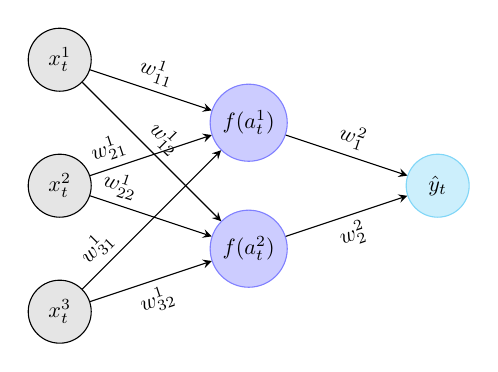
\begin{tikzpicture}[nef, scale=0.8, every node/.style={scale=0.8}]
          % Input Layer
          \node[input node] (x1) at (0, 2) {$x_t^1$};
          \node[input node] (x2) at (0, 0) {$x_t^2$};
          \node[input node] (x3) at (0, -2) {$x_t^3$};         
          % Hidden Layer
          \node[hidden node] (h1) at (3, 1) {$f(a_t^1)$};
          \node[hidden node] (h2) at (3, -1) {$f(a_t^2)$};      
          % Output Layer
          \node[output node] (y) at (6, 0) {$\hat{y}_t$};          
          % Connections
          \draw[arrow] (x1) -- node[above, sloped] {$w_{11}^1$} (h1);
          \draw[arrow] (x1) -- node[above, sloped] {$w_{12}^1$} (h2);        
          \draw[arrow] (x2) -- node[above, sloped, pos=0.2] {$w_{21}^1$} (h1);
          \draw[arrow] (x2) -- node[above, sloped, pos=0.2] {$w_{22}^1$} (h2);
          \draw[arrow] (x3) -- node[above, sloped, pos=0.2] {$w_{31}^1$} (h1);
          \draw[arrow] (x3) -- node[below, sloped] {$w_{32}^1$} (h2);        
          \draw[arrow] (h1) -- node[above, sloped] {$w_1^2$} (y);
          \draw[arrow] (h2) -- node[below, sloped] {$w_2^2$} (y);
        \end{tikzpicture}\\
        \textbf{NN Matrix Algebra}
        $
          \begin{bmatrix}
            x_t^1 & x_t^2 & x_t^3
          \end{bmatrix}
          \begin{bmatrix}
            w_{11}^1 & w_{12}^1 \\
            w_{21}^1 & w_{22}^1 \\
            w_{31}^1 & w_{32}^1
          \end{bmatrix}
          =
          \begin{bmatrix}
            a_t^1 & a_t^2
          \end{bmatrix}
        $
        $
          \begin{bmatrix}
            f(a_t^{1}) & f(a_{t}^{2})
          \end{bmatrix}
          \begin{bmatrix}
            w_1^2 \\
            w_2^2
          \end{bmatrix}
          = \hat{y}_t
        $
      \end{column}
    \end{columns}
  \end{frame}

  \section{Conclusion}
  \begin{frame}{Conclusion}
    \begin{itemize}
      \item That's all
    \end{itemize}
  \end{frame}

  %% Redefining footer after conclusion to not have total frame number
  \setbeamertemplate{footline}{
    \hbox{
      \setbeamercolor{footercolor}{bg = white, fg = white!50!black}
      \begin{beamercolorbox}[wd = 0.333333\paperwidth,ht = 2.25ex, dp = 2ex, left]{footercolor}%
        \hspace*{2ex} \insertshortauthor\hspace*{0.5ex}  (\insertshortinstitute)
      \end{beamercolorbox}%
      \begin{beamercolorbox}[wd = 0.333333\paperwidth,ht = 2.25ex, dp = 2ex, center]{footercolor}%
        \insertshorttitle
      \end{beamercolorbox}%
      \begin{beamercolorbox}[wd = 0.333333\paperwidth,ht = 2.25ex,dp = 2ex,right]{footercolor}%
        % \insertframenumber{}
        %% Uncomment the line below if you wish to show the total frame number
        % / \inserttotalframenumber
        \hspace*{4ex} 
      \end{beamercolorbox}
    }
    \vskip0pt
  }

  %% The frame number of all slides in the following group are considered as empty in
  %%the actual PDF, but has the original definition in the PDF metadata 
  \begingroup
    \def\insertframenumber{\texorpdfstring{\relax}{\sidepanenumber}}
    \begin{frame}[noframenumbering]
      \begin{center}
        \Huge{\textcolor{basecolor}{Thank you!}}\\
        \vspace{6mm}
        \normalsize{
          \href{mailto:your@email.address}{your@email.address}\\
          \vspace{3mm}
          \href{https://google.com/}{https://yourwebsite.com/}
        }
      \end{center}
    \end{frame}

    %% Creating references slides
    %% Making references font size to be tiny
    \renewcommand*{\bibfont}{\normalfont\tiny}
    \begin{frame}[t, noframenumbering, allowframebreaks]{References} % add option allowframebreaks if long reference list
      \printbibliography
    \end{frame}

    %% Additional slides that are linked
    %% Declaring empty section to serve as the appendix section without hiding the navigation bar
    \section*{}
    \begin{frame}[noframenumbering]{Appendix \hfill\hyperlink{introduction}{\beamerbutton{Back to Introduction}}}\label{app}
    \end{frame}
  \endgroup
\end{document}